\documentclass[xcolor=svgnames, 10pt, handout]{beamer}

\usepackage{soul}
\usepackage[utf8]{inputenc}
\usepackage[T1]{fontenc}
\usepackage[english]{babel}

%\usepackage{verbatim}

\usepackage[export]{adjustbox}

\usepackage{
    amsmath,
    amsfonts,
    etex,
    fancyvrb,
    graphicx,
    multicol,
    pifont,
    setspace,
    soul,
    spverbatim,
    textcomp,
    xcolor,
    xspace
}

\usepackage{tikz}
\usetikzlibrary{shadows}

%%%SETUP%%%
\hypersetup{
     colorlinks = true,
     linkcolor = blue,
     anchorcolor = blue,
     citecolor = blue,
     filecolor = blue,
     urlcolor = blue
     }
     
%%%THEOREMS%%%
\theoremstyle{example}
\newtheorem*{exercise}{Exercise}
\newtheorem*{question}{Question}
\newtheorem*{answer}{\emph{Answer}}
\newtheorem*{notation}{Notation}

%%%TWEAKS%%%
\setlength\arraycolsep{4pt}
\addtolength\fboxsep{10pt}
\setstretch{1.4}
\setbeamersize{description width=3em}
\setbeamersize{text margin left=.5cm,text margin right=.5cm} 
\renewcommand{\emph}{\alert}
\renewcommand{\arraystretch}{1.2}
\renewcommand{\tabcolsep}{4pt}
\setbeamercolor{alerted text}{fg=magenta}


\graphicspath{{img/}}

%for straight quotes in verbatim:
\usepackage{upquote,textcomp}

%turn off navigation symbols
\beamertemplatenavigationsymbolsempty
\setbeamertemplate{footline}[frame number]

%title page

\author
  [Dr.\ Irene Vrbik]
  {Dr.\ Irene Vrbik}

\date
  {}

\institute
  {University of British Columbia Okanagan \newline \texttt{irene.vrbik@ubc.ca}}
  
\definecolor{iyellow}{RGB}{255, 162, 23}
\definecolor{sgreen}{RGB}{118, 191, 138}

\newcommand{\yellow}[1]{\textcolor{iyellow}{#1}}
\newcommand{\red}[1]{\textcolor{red}{#1}}
\newcommand{\green}[1]{\textcolor{ForestGreen}{#1}}
\newcommand{\blue}[1]{{\textcolor{blue}{#1}}}
\newcommand{\orange}[1]{{\textcolor{orange}{#1}}}
\newcommand{\bblue}[1]{\textcolor{SteelBlue!90!gray}{#1}} % beamer blue
\newcommand{\purple}[1]{{\textcolor{purple}{#1}}}

\newcommand{\el}{\\[1em]\pause}
\newcommand{\nl}{\\[1em]}
\newcommand{\define}[1]{\textbf{\textcolor{orange}{#1}}}

%\newcommand{\answer}[1]{\textit{\textbf{\textcolor{iyellow}{#1}}}}

\newcommand{\command}[1]{\texttt{\textbf{\textcolor{DarkMagenta}{#1}}}}
\newcommand{\ipic}[2]{\includegraphics[width={#2}\textwidth]{#1}}
\newcommand{\cell}[1]{{\sf \textbf{\textcolor{DarkMagenta}{#1}}}}
\newcommand{\ra}{$\rightarrow$}

\newcommand{\ft}[1]{\frametitle{#1}}


\newenvironment{allintypewriter}{\ttfamily}{\par}
\newcommand{\bs}{$\backslash$}

\newcommand*\keystroke[1]{%
  \tikz[baseline=(key.base)]
    \node[%
      draw,
      fill=white,
      drop shadow={shadow xshift=0.25ex,shadow yshift=-0.25ex,fill=black,opacity=0.75},
      rectangle,
      rounded corners=2pt,
      inner sep=1pt,
      line width=0.5pt,
      font=\scriptsize\sffamily
    ](key) {#1\strut}
  ;
}

% timed answer
\newcommand{\tans}[2]{\textbf<#1>{\textit<#1>{{\color<#1>{iyellow}{#2}}}}}


\makeatletter
\g@addto@macro\normalsize{%
  \setlength\abovedisplayskip{0.4em}
  \setlength\belowdisplayskip{0.4em}
  \setlength\abovedisplayshortskip{0.2em}
  \setlength\belowdisplayshortskip{0.2em}
}
\makeatother


\newcommand{\cmark}{{\Large\color{green}\ding{51}}}%
\newcommand{\xmark}{{\Large\color{red}\ding{55}}}%

\newcommand{\pcmark}{\onslide<+->{\cmark}}
\newcommand{\pxmark}{\onslide<+->{\xmark}}

\newcommand{\by}{\overline{y}}
\newcommand{\ty}{\tilde{y}}

\title
  [R]
  {R part II}
  \subtitle{Data Analysis with R}


\begin{document}


\maketitle


%%%%%%%%%%%%%%%%%%%%%%%%%%%%%%%%%%%%%%%%%%%%%%%%%%%%%%%%%%%%%%%%%%%%%%%%%%%%%%%%%%%%%%%%%%%%%%%%%%%%
\begin{frame}[fragile]{Vector}
A \emph{vector} is an indexed list of data of any type.
\vfill
Create vectors using a colon or \texttt{seq()} (R's version of range)
\begin{Verbatim}[commandchars=\\\{\}, xleftmargin=2em]
> 1:10
[1]  1  2  3  4  5  6  7  8  9 10
> seq(5, 1, by = -0.5 )
[1] 5.0 4.5 4.0 3.5 3.0 2.5 2.0 1.5 1.0
\end{Verbatim}
\vfill
Create an empty vector with \texttt{c()} or fill it by specifying elements.
\begin{Verbatim}[commandchars=\\\{\}, xleftmargin=2em]
> c()
NULL
> c(4, 3, 5, 'a', 'd')
[1] "4" "3" "5" "a" "d"
\end{Verbatim}
\end{frame}
%%%%%%%%%%%%%%%%%%%%%%%%%%%%%%%%%%%%%%%%%%%%%%%%%%%%%%%%%%%%%%%%%%%%%%%%%%%%%%%%%%%%%%%%%%%%%%%%%%%%


%%%%%%%%%%%%%%%%%%%%%%%%%%%%%%%%%%%%%%%%%%%%%%%%%%%%%%%%%%%%%%%%%%%%%%%%%%%%%%%%%%%%%%%%%%%%%%%%%%%%
\begin{frame}[fragile]{Vector}
Access elements in a vector using \texttt{[ ]}
\begin{Verbatim}[commandchars=\\\{\}, xleftmargin=2em]
> myVector = c(4, 3, 5, 'a', 'd')
> myVector[i]  #Returns the ith element of myVector
> myVector[1]
[1] "4"
\end{Verbatim}
\end{frame}


\begin{frame}[fragile]{ Vectors}
We could also name vectors (similar to Python's dictionaries)
\begin{Verbatim}[commandchars=\\\{\}, xleftmargin=2em]
> names(myVector) <- c("first", "second", "third",
"fourth","fifth")
> myVector["first"]
first 
  "4" 
\end{Verbatim}
\end{frame}


%%%%%%%%%%%%%%%%%%%%%%%%%%%%%%%%%%%%%%%%%%%%%%%%%%%%%%%%%%%%%%%%%%%%%%%%%%%%%%%%%%%%%%%%%%%%%%%%%%%%


%%%%%%%%%%%%%%%%%%%%%%%%%%%%%%%%%%%%%%%%%%%%%%%%%%%%%%%%%%%%%%%%%%%%%%%%%%%%%%%%%%%%%%%%%%%%%%%%%%%%
\begin{frame}[fragile]{Vectors in R}
\begin{question}
Which (if any) of the following statements are true?
\begin{enumerate}
\item Vectors in R are indexed from 0.  \onslide<+-> \pxmark
\item \texttt{1:10} creates a vector of ten numbers. \pcmark
\item A vector may have data value of different types. \pxmark
\item If \texttt{data <- 1:5} then \texttt{data[2] + data[3] = 3}. \pxmark
\end{enumerate}
\end{question}
\end{frame}
%%%%%%%%%%%%%%%%%%%%%%%%%%%%%%%%%%%%%%%%%%%%%%%%%%%%%%%%%%%%%%%%%%%%%%%%%%%%%%%%%%%%%%%%%%%%%%%%%%%%


%%%%%%%%%%%%%%%%%%%%%%%%%%%%%%%%%%%%%%%%%%%%%%%%%%%%%%%%%%%%%%%%%%%%%%%%%%%%%%%%%%%%%%%%%%%%%%%%%%%%
\begin{frame}[fragile]{Matrices}
A \emph{matrix} is a structure of rows and columns where each data value is the same data type.  All rows must have the same length.  All columns must have the same length.
\vfill
Create a matrix from the vector \texttt{x} using \texttt{matrix()}.
\begin{Verbatim}[commandchars=\\\{\}, xleftmargin=2em]
> matrix(x, nrow=5, ncol=3, byrow=False)
# Starts at [1,1] and fills the column first before going to
# next column.
# Need to only specify ncol or nrow.
\end{Verbatim}
\vfill
Access elements using \texttt{[row, col]}.  Leaving one of them blank returns the whole row or column.
\begin{Verbatim}[commandchars=\\\{\}, xleftmargin=2em]
> myMatrix[i, j]  #Returns ith row and jth column.
\end{Verbatim}
\end{frame}
%%%%%%%%%%%%%%%%%%%%%%%%%%%%%%%%%%%%%%%%%%%%%%%%%%%%%%%%%%%%%%%%%%%%%%%%%%%%%%%%%%%%%%%%%%%%%%%%%%%%


%%%%%%%%%%%%%%%%%%%%%%%%%%%%%%%%%%%%%%%%%%%%%%%%%%%%%%%%%%%%%%%%%%%%%%%%%%%%%%%%%%%%%%%%%%%%%%%%%%%%
\begin{frame}[fragile]{Matrices and Vectors}
\vfill
Append a vector to a matrix as a row using \texttt{rbind()}
\begin{Verbatim}[commandchars=\\\{\}, xleftmargin=2em]
> myMatrix = rbind(myMatrix, vec)
\end{Verbatim}
\vfill
Append a vector to a matrix as a column using \texttt{cbind()}
\begin{Verbatim}[commandchars=\\\{\}, xleftmargin=2em]
> myMatrix = cbind(myMatrix, vec)
\end{Verbatim}
\vfill
\end{frame}


\begin{frame}[fragile]{Matrices and Vectors}
We could also name the columns are rows of a matrix:
\begin{Verbatim}[commandchars=\\\{\}, xleftmargin=2em]
> mat1 <- matrix(1:12, nrow=3)
> colnames(mat1) <- c("col1", "col2", "col3", "col4")
> rownames(mat1) <- c("row1", "row2", "row3")
> mat1["row1",] # same as mat[1,]
col1 col2 col3 col4 
   1    4    7   10 
> mat1$col3 # won't work (can only use $ on data.frames)
Error in mat1$col3 : $ operator is invalid for atomic vectors
\end{Verbatim}
\end{frame}
%%%%%%%%%%%%%%%%%%%%%%%%%%%%%%%%%%%%%%%%%%%%%%%%%%%%%%%%%%%%%%%%%%%%%%%%%%%%%%%%%%%%%%%%%%%%%%%%%%%%


%%%%%%%%%%%%%%%%%%%%%%%%%%%%%%%%%%%%%%%%%%%%%%%%%%%%%%%%%%%%%%%%%%%%%%%%%%%%%%%%%%%%%%%%%%%%%%%%%%%%
\begin{frame}[fragile]{Lists}
A \emph{list} is an ordered collection of objects of \emph{any} type.
\vfill
Create a list using \texttt{list()}.  Specify names of elements by using \texttt{name =} inside the brackets.
\begin{Verbatim}[commandchars=\\\{\}, xleftmargin=2em]
> myList = list(x=1:4, y=c('a', 'b'))
#Creates a list with two elements x and y
\end{Verbatim}
\vfill
Access elements using the double square brackets.
\begin{Verbatim}[commandchars=\\\{\}, xleftmargin=2em]
> myList[[2]]   # Returns the 2nd item of list (y)
> myList[['x']] #Returns item with the name x.
> myList$x #Returns item with the name x (no quotes)
\end{Verbatim}
\end{frame}
%%%%%%%%%%%%%%%%%%%%%%%%%%%%%%%%%%%%%%%%%%%%%%%%%%%%%%%%%%%%%%%%%%%%%%%%%%%%%%%%%%%%%%%%%%%%%%%%%%%%


%%%%%%%%%%%%%%%%%%%%%%%%%%%%%%%%%%%%%%%%%%%%%%%%%%%%%%%%%%%%%%%%%%%%%%%%%%%%%%%%%%%%%%%%%%%%%%%%%%%%
\begin{frame}[fragile]{Lists and Matrices in R}
\begin{question}
Which (if any) of the following statements are true?
\begin{enumerate}
\item Data values in a list may be of different types. \onslide<+-> \pcmark 
\item In a matrix, the number of rows and columns must be the same. \pxmark
\item Given matrix \texttt{m, m[2]} would return an error. \pxmark 
\item Given matrix \texttt{m, m[,2]} would return all data in column 2. \pcmark
\end{enumerate}
\end{question}
\end{frame}
%%%%%%%%%%%%%%%%%%%%%%%%%%%%%%%%%%%%%%%%%%%%%%%%%%%%%%%%%%%%%%%%%%%%%%%%%%%%%%%%%%%%%%%%%%%%%%%%%%%%


%%%%%%%%%%%%%%%%%%%%%%%%%%%%%%%%%%%%%%%%%%%%%%%%%%%%%%%%%%%%%%%%%%%%%%%%%%%%%%%%%%%%%%%%%%%%%%%%%%%%
\begin{frame}[fragile]
\begin{question}
Create a list called \texttt{grades} and add the following elements
\begin{enumerate}
\item Name (first name and last name),
\item Student number,
\item Assignment grades (multiple entries), and
\item Midterm grade.
\end{enumerate}
\end{question}
\end{frame}
%%%%%%%%%%%%%%%%%%%%%%%%%%%%%%%%%%%%%%%%%%%%%%%%%%%%%%%%%%%%%%%%%%%%%%%%%%%%%%%%%%%%%%%%%%%%%%%%%%%%


%%%%%%%%%%%%%%%%%%%%%%%%%%%%%%%%%%%%%%%%%%%%%%%%%%%%%%%%%%%%%%%%%%%%%%%%%%%%%%%%%%%%%%%%%%%%%%%%%%%%
\begin{frame}[fragile]{Data Frame}
\vfill
A \emph{data frame} is similar to a matrix but the columns can have different data types.  Note these data frames are quite common and have uniform length of rows and columns.
\vfill
To create a data frame by using \texttt{data.frame()}, specify names of variables within the brackets:
\begin{Verbatim}[commandchars=\\\{\}, xleftmargin=2em]
> myDF = data.frame(x = c(1:3), y = (2:4))
\end{Verbatim}
\vfill
To convert a matrix into a \texttt{data.frame} using \texttt{as.data.frame()}.
\begin{Verbatim}[commandchars=\\\{\}, xleftmargin=2em]
> myDF = as.data.frame(myMatrix)
\end{Verbatim}
\vfill
\end{frame}
%%%%%%%%%%%%%%%%%%%%%%%%%%%%%%%%%%%%%%%%%%%%%%%%%%%%%%%%%%%%%%%%%%%%%%%%%%%%%%%%%%%%%%%%%%%%%%%%%%%%


%%%%%%%%%%%%%%%%%%%%%%%%%%%%%%%%%%%%%%%%%%%%%%%%%%%%%%%%%%%%%%%%%%%%%%%%%%%%%%%%%%%%%%%%%%%%%%%%%%%%
\begin{frame}[fragile]{Accessing Data in Data Frames}

Access elements using \texttt{[row, col]} or \verb|$variable_name|.
\begin{Verbatim}[commandchars=\\\{\}, xleftmargin=2em]
> myDF[i, j]           #ith row and jth column
> myDF\$x               #returns the column labelled x
\end{Verbatim}

Add new columns called \texttt{vec} into the data frame use in \verb|$|.
\begin{Verbatim}[commandchars=\\\{\}, xleftmargin=2em]
> myDF$new_col = vec   #Adds vec as new_col
\end{Verbatim}

\end{frame}
%%%%%%%%%%%%%%%%%%%%%%%%%%%%%%%%%%%%%%%%%%%%%%%%%%%%%%%%%%%%%%%%%%%%%%%%%%%%%%%%%%%%%%%%%%%%%%%%%%%%


%%%%%%%%%%%%%%%%%%%%%%%%%%%%%%%%%%%%%%%%%%%%%%%%%%%%%%%%%%%%%%%%%%%%%%%%%%%%%%%%%%%%%%%%%%%%%%%%%%%%
\begin{frame}[fragile]{Factors}
\emph{Factors} are used for qualitative groups/categories (i.e. male/female).  Use \verb|as.factor()| to turn a vector or \verb|data.frame| column into a factor.
\vfill
\begin{Verbatim}[commandchars=\\\{\}, xleftmargin=2em]
mFyFactor = as.factor(x)
myDF\$x = as.factor(myDF\$x)
\end{Verbatim}
\vfill
Access elements using \verb|[ ]|:
\begin{Verbatim}[commandchars=\\\{\}, xleftmargin=2em]
myFactor[i]    #Returns ith element
\end{Verbatim}
\vfill
Can use \verb|class()| or \verb|str()| to gain information about the type and/or structure of your variable/data. \verb|str()|  gives me detail.
\vfill
\end{frame}
%%%%%%%%%%%%%%%%%%%%%%%%%%%%%%%%%%%%%%%%%%%%%%%%%%%%%%%%%%%%%%%%%%%%%%%%%%%%%%%%%%%%%%%%%%%%%%%%%%%%


%%%%%%%%%%%%%%%%%%%%%%%%%%%%%%%%%%%%%%%%%%%%%%%%%%%%%%%%%%%%%%%%%%%%%%%%%%%%%%%%%%%%%%%%%%%%%%%%%%%%
\begin{frame}[fragile]
\begin{question}
Which (if any) of the following are true?
\begin{enumerate}
\item Matrices must have the same number of rows as columns. \onslide<+-> \pxmark
\item Vectors must contain only one data type. \pcmark
\item \st{A factor can contain only characters.} 
% \footnote{this isn't a very good question} 
\textit{While we can use numbers to represent the factors (eg. 0 = male, 1 = female) they will be treated as characters in R. }
\item A  \emph{data frame's} columns can be of varying length. \pxmark
\end{enumerate}
\end{question}
\end{frame}
%%%%%%%%%%%%%%%%%%%%%%%%%%%%%%%%%%%%%%%%%%%%%%%%%%%%%%%%%%%%%%%%%%%%%%%%%%%%%%%%%%%%%%%%%%%%%%%%%%%%


%%%%%%%%%%%%%%%%%%%%%%%%%%%%%%%%%%%%%%%%%%%%%%%%%%%%%%%%%%%%%%%%%%%%%%%%%%%%%%%%%%%%%%%%%%%%%%%%%%%%
\begin{frame}[fragile]{Subsets}
Subsetting is used to extract data with particular values.
\vfill
\begin{Verbatim}[xleftmargin=2em, xrightmargin=1.5em, frame=single, label=Syntax in R, framesep=0.5em]
subset(data, condition)
# if we want to check two conditions:
subset(data, condition1 & condition2)
\end{Verbatim}
\vfill
\begin{Verbatim}[xleftmargin=2em, xrightmargin=1.5em, frame=single, label=Example in R, framesep=0.5em]
cars_bc = subset(cars, prov == 'BC')
\end{Verbatim}
\vfill
\end{frame}
%%%%%%%%%%%%%%%%%%%%%%%%%%%%%%%%%%%%%%%%%%%%%%%%%%%%%%%%%%%%%%%%%%%%%%%%%%%%%%%%%%%%%%%%%%%%%%%%%%%%


%%%%%%%%%%%%%%%%%%%%%%%%%%%%%%%%%%%%%%%%%%%%%%%%%%%%%%%%%%%%%%%%%%%%%%%%%%%%%%%%%%%%%%%%%%%%%%%%%%%%
\begin{frame}[fragile]
\begin{question}
\begin{enumerate}
\item Create a \emph{data frame} \verb|mydata| with the following column names/data:
\begin{enumerate}
\item \verb|id| -- numbers one to 5.
\item \verb|location| -- ``BC'', ``BC'', ``AB'', ``MB'', ``BC''.
\item \verb|value| -- 10, 20, 30, 40, 50.
\item Make location a factor.
\end{enumerate}
\item Add one more column to your data frame that is a factor
\begin{enumerate}
\item \verb|success| -- ``Y'', ``N'', `N'', `N'', ``Y''.
\end{enumerate}
\item Display only the data from BC and value $\geq 20$.
\end{enumerate}
\end{question}

\end{frame}
%%%%%%%%%%%%%%%%%%%%%%%%%%%%%%%%%%%%%%%%%%%%%%%%%%%%%%%%%%%%%%%%%%%%%%%%%%%%%%%%%%%%%%%%%%%%%%%%%%%%


%%%%%%%%%%%%%%%%%%%%%%%%%%%%%%%%%%%%%%%%%%%%%%%%%%%%%%%%%%%%%%%%%%%%%%%%%%%%%%%%%%%%%%%%%%%%%%%%%%%%
\begin{frame}[fragile]{Visualizing Data in R}
R supports several graphing libraries to produce graphs for qualitative and quantitative data including bar charts, histograms, and box plots.
\vfill
We will use the package \verb|ggplot2.gg| stands for Grammar of Graphics.
\vfill
See the \href{https://www.rstudio.com/wp-content/uploads/2015/03/ggplot2-cheatsheet.pdf}{\red{ggplot cheatsheet}}
\end{frame}


\begin{frame}[fragile]{Visualizing Data in R}

To install \texttt{Tools $\to$ Install Packages}\ldots Then input \verb|ggplot2|.
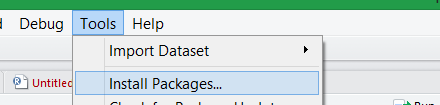
\includegraphics[width=0.5\textwidth]{images/debug}
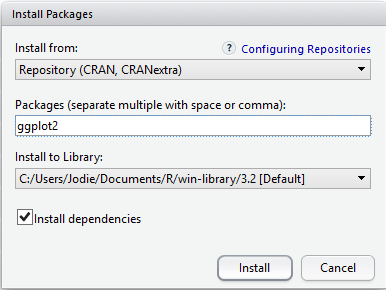
\includegraphics[width=.4\textwidth]{images/installpackage}

Or (and this would be my preferred method) type the command:
\begin{Verbatim}[label=Install package]
install.packages("ggplot2")
\end{Verbatim}
To load that library into your working session type:
\begin{Verbatim}[label=load package]
load("ggplot2") # quotes not necessary
\end{Verbatim}

\end{frame}
%%%%%%%%%%%%%%%%%%%%%%%%%%%%%%%%%%%%%%%%%%%%%%%%%%%%%%%%%%%%%%%%%%%%%%%%%%%%%%%%%%%%%%%%%%%%%%%%%%%%


%%%%%%%%%%%%%%%%%%%%%%%%%%%%%%%%%%%%%%%%%%%%%%%%%%%%%%%%%%%%%%%%%%%%%%%%%%%%%%%%%%%%%%%%%%%%%%%%%%%%
\begin{frame}[fragile]{Graphs for Qualitative Data: Frequency Tables}
\emph{Frequency tables} summarize the number of observations in each group.
\vfill
\begin{Verbatim}[xleftmargin=2em, xrightmargin=1.5em, frame=single, numbers=left, label=Frequency Table, framesep=0.5em]
> table(Auto$origin)
  1   2   3
245  68  79
\end{Verbatim}
\vfill
\end{frame}
%%%%%%%%%%%%%%%%%%%%%%%%%%%%%%%%%%%%%%%%%%%%%%%%%%%%%%%%%%%%%%%%%%%%%%%%%%%%%%%%%%%%%%%%%%%%%%%%%%%%


%%%%%%%%%%%%%%%%%%%%%%%%%%%%%%%%%%%%%%%%%%%%%%%%%%%%%%%%%%%%%%%%%%%%%%%%%%%%%%%%%%%%%%%%%%%%%%%%%%%%
\begin{frame}[fragile]{Graphs for Qualitative Data: Bar Charts}
\begin{multicols}{2}
\emph{Bar charts} have each group along the $x$-axis and a vertical bar with the height representing the number of observations of each group.
\vfill
Using the dataset {\tt Auto} in the ISLR package.
\vfill
\newpage
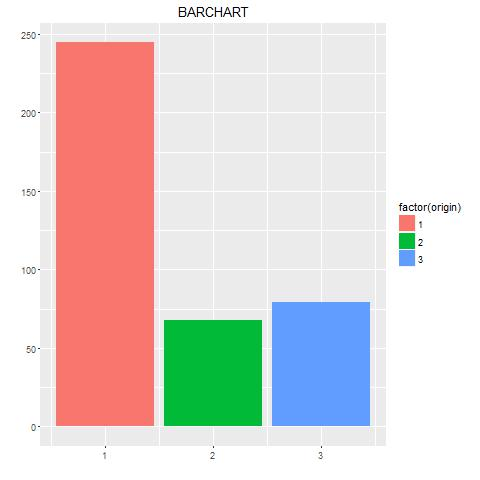
\includegraphics[width=0.4\textwidth]{images/barchart}
\end{multicols}
\begin{Verbatim}[xleftmargin=2em, xrightmargin=1.5em, frame=single, numbers=left, label=Frequency Table, framesep=0.5em]
ggplot(Auto, aes(x=origin))
+ geom_bar(aes(fill=factor(origin)))
+ xlab("") + ylab("") + ggtitle("BARCHART")
\end{Verbatim}
\end{frame}
%%%%%%%%%%%%%%%%%%%%%%%%%%%%%%%%%%%%%%%%%%%%%%%%%%%%%%%%%%%%%%%%%%%%%%%%%%%%%%%%%%%%%%%%%%%%%%%%%%%%


%%%%%%%%%%%%%%%%%%%%%%%%%%%%%%%%%%%%%%%%%%%%%%%%%%%%%%%%%%%%%%%%%%%%%%%%%%%%%%%%%%%%%%%%%%%%%%%%%%%%
\begin{frame}[fragile]{Graphs for Quantitative Data: Histogram}
\begin{multicols}{2}

A \emph{histogram} is similar to a bar chart, but the $x$-axis is divided into bins.
\vfill
The variable of interest is on the $x$-axis and the $y$-axis represents count of observations within each bin.
\vfill
Visualizes the data distribution.
\vfill
\newpage

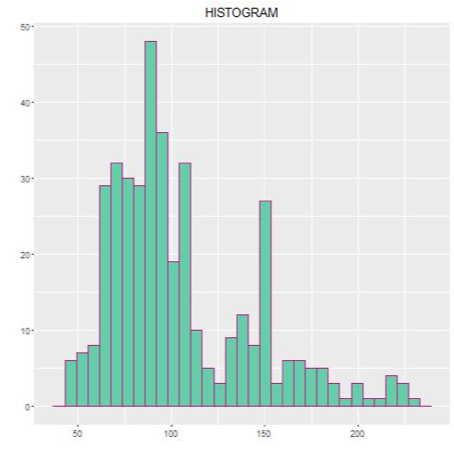
\includegraphics[width=0.4\textwidth]{images/hist}
\end{multicols}

\begin{Verbatim}[xleftmargin=.5em, xrightmargin=.5em, frame=single, label=Histogram Example, framesep=0.5em, fontsize=\small]
ggplot(Auto, aes(x=horsepower))
+ geom_histogram(color='mediumvioletred', fill='mediumaquarmarine')
+ xlab("") + ylab("") + ggtitle("HISTOGRAM")
\end{Verbatim}
\end{frame}
%%%%%%%%%%%%%%%%%%%%%%%%%%%%%%%%%%%%%%%%%%%%%%%%%%%%%%%%%%%%%%%%%%%%%%%%%%%%%%%%%%%%%%%%%%%%%%%%%%%%


%%%%%%%%%%%%%%%%%%%%%%%%%%%%%%%%%%%%%%%%%%%%%%%%%%%%%%%%%%%%%%%%%%%%%%%%%%%%%%%%%%%%%%%%%%%%%%%%%%%%
\begin{frame}[fragile]{Graphs for Quantitative Data: Boxplot}
A \emph{boxplot} is a visualization of the five number summary.
\begin{multicols}{2}
\begin{enumerate}
\item Groups along the $x$-axis.

\item Data values along the $y$-axis.

\item Lowest and highest points are the min and max of the data respectively.

\item Bottom of box is Q1 and top is Q3.

\item Median is represented as the bar inside the box.

\item Single points represent outliers.
\end{enumerate}
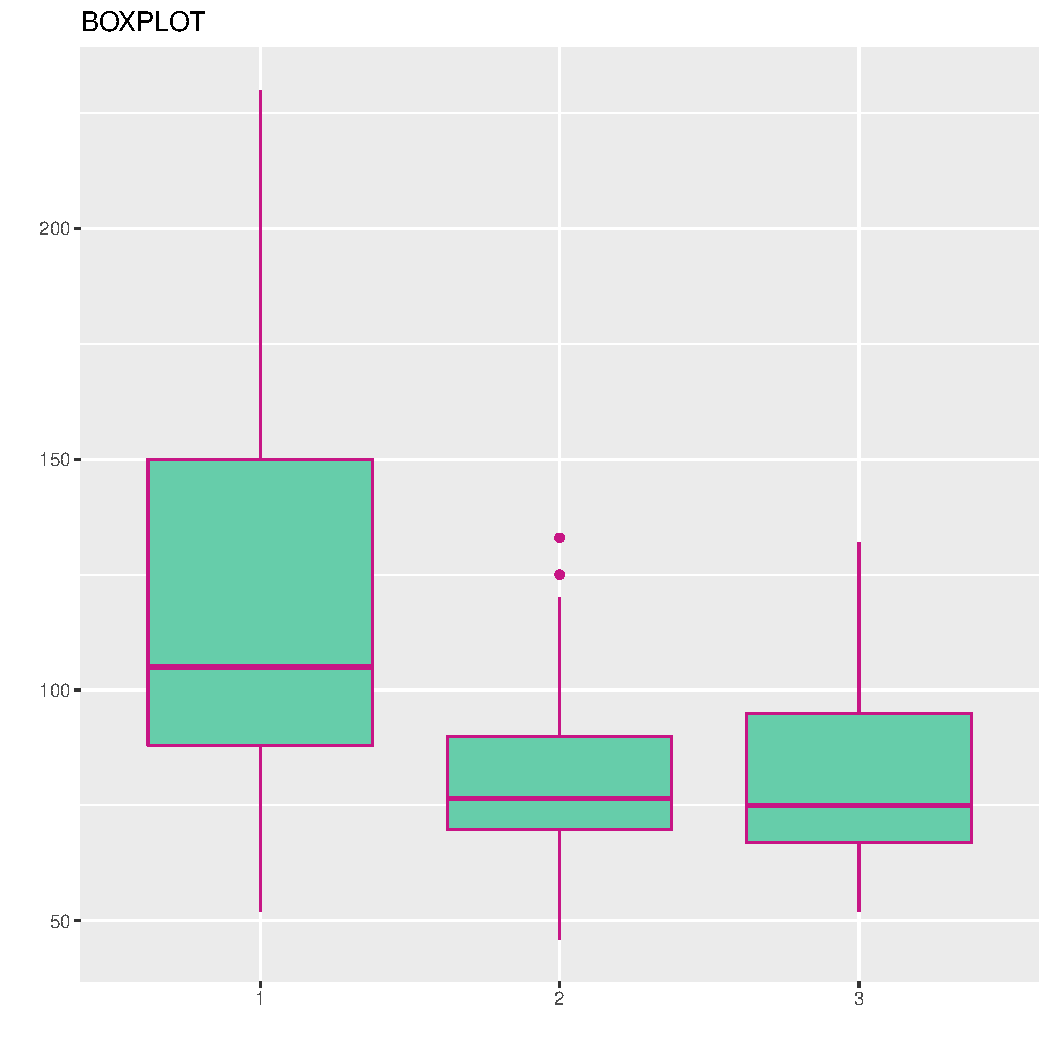
\includegraphics[width=0.4\textwidth]{images/boxplot}
\end{multicols}
\end{frame}
%%%%%%%%%%%%%%%%%%%%%%%%%%%%%%%%%%%%%%%%%%%%%%%%%%%%%%%%%%%%%%%%%%%%%%%%%%%%%%%%%%%%%%%%%%%%%%%%%%%%


%%%%%%%%%%%%%%%%%%%%%%%%%%%%%%%%%%%%%%%%%%%%%%%%%%%%%%%%%%%%%%%%%%%%%%%%%%%%%%%%%%%%%%%%%%%%%%%%%%%%
\begin{frame}[fragile]{Boxplot Example Code}
\begin{Verbatim}[xleftmargin=.5em, xrightmargin=.5em, frame=single, label=Boxplot Example, framesep=0.5em, fontsize=\small]
ggplot(Auto, aes(x=factor(origin), y=horsepower))
+ geom_boxplot(color='mediumvioletred', fill='mediumaquamarine')
+ xlab("") + ylab("") + ggtitle("BOXPLOT")
\end{Verbatim}
\end{frame}
%%%%%%%%%%%%%%%%%%%%%%%%%%%%%%%%%%%%%%%%%%%%%%%%%%%%%%%%%%%%%%%%%%%%%%%%%%%%%%%%%%%%%%%%%%%%%%%%%%%%


%%%%%%%%%%%%%%%%%%%%%%%%%%%%%%%%%%%%%%%%%%%%%%%%%%%%%%%%%%%%%%%%%%%%%%%%%%%%%%%%%%%%%%%%%%%%%%%%%%%%
\begin{frame}[fragile]{Graphs for Quantitative Data: ECDF}
\begin{multicols}{2}
An \emph{empirical cumulative distribution function (ECDF) plot} shows values along the $x$-axis and quantiles along the $y$-axis.
\vfill
Each data point is plotted along with its corresponding quantile.
\vfill
\newpage
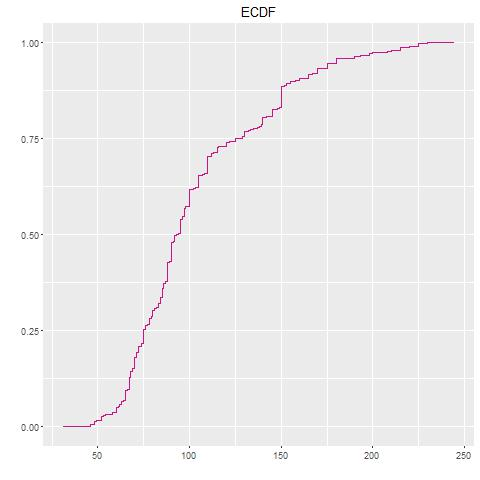
\includegraphics[width=0.4\textwidth]{images/ecdf}
\end{multicols}
\vfill
\begin{Verbatim}[xleftmargin=.5em, xrightmargin=.5em, frame=single, label=Boxplot Example, framesep=0.5em, fontsize=\small]
ggplot(Auto, aes(x=horsepower))
+ stat_ecdf(color='mediumvioletred')
+ xlab("") + ylab("") + ggtitle("ECDF")
\end{Verbatim}
\end{frame}
%%%%%%%%%%%%%%%%%%%%%%%%%%%%%%%%%%%%%%%%%%%%%%%%%%%%%%%%%%%%%%%%%%%%%%%%%%%%%%%%%%%%%%%%%%%%%%%%%%%%


%%%%%%%%%%%%%%%%%%%%%%%%%%%%%%%%%%%%%%%%%%%%%%%%%%%%%%%%%%%%%%%%%%%%%%%%%%%%%%%%%%%%%%%%%%%%%%%%%%%%
\begin{frame}[fragile]
\begin{question}
Which (if any)  of the following are true?
\begin{enumerate}
\item Bar charts and histograms will work for the same variables. \onslide<+-> \pxmark
\item Boxplots show a five number summary. \pcmark
\item Variables type does not matter, any graph can be used. \pxmark
\item Histograms can give an idea of the distribution of a variable. \pcmark
\end{enumerate}
\end{question}
\end{frame}
%%%%%%%%%%%%%%%%%%%%%%%%%%%%%%%%%%%%%%%%%%%%%%%%%%%%%%%%%%%%%%%%%%%%%%%%%%%%%%%%%%%%%%%%%%%%%%%%%%%%


%%%%%%%%%%%%%%%%%%%%%%%%%%%%%%%%%%%%%%%%%%%%%%%%%%%%%%%%%%%%%%%%%%%%%%%%%%%%%%%%%%%%%%%%%%%%%%%%%%%%
%\begin{frame}[fragile]
%\begin{question}
%\begin{enumerate}
%\item Using the car data from the \verb|data.frame| example, create a bar chart for the variable \verb|prov|.
%\item Use the cars data and create a histogram of any variable.
%\item Create a boxplot for the variable of your choice.
%\begin{enumerate}
%\item What are the median and minimum values? Can you estimate the IQR?
%\end{enumerate}
%\item Make an ECDF for the variable of your choice.
%\begin{enumerate}
%\item Recalling that Q1, median, and Q3 are the 0.25, 0.5, and 0.75th quantiles, what is yoru best guess at these values from reading off of the graphs?
%\end{enumerate}
%\end{enumerate}
%\end{question}
%\end{frame}
%%%%%%%%%%%%%%%%%%%%%%%%%%%%%%%%%%%%%%%%%%%%%%%%%%%%%%%%%%%%%%%%%%%%%%%%%%%%%%%%%%%%%%%%%%%%%%%%%%%%%


\end{document}
%%%%%%%%%%%%%%%%%%%%%%%%%%%%%%%%%%%%%%%%%%%%%%%%%%%%%%%%%%%%%%%%%%%%%%%%%%%%%%%%%%%%%%%%%%%%%%%%%%%%
